\section{Introduction}
    In the Vortex \ae ther Model (VAM), gravitation and quantum phenomena are reformulated through the topology and dynamics of vorticity in an incompressible, inviscid fluid-like \ae ther. This article derives a formal connection between classical defect theory---dislocations and disclinations in condensed matter physics---and VAM's vortex core structures using the language of Cartan geometry. Inspired by recent developments \cite{kobayashi2025}, we reinterpret torsion and curvature within the Cartan structure equations in terms of swirl density and topological vortex curvature. Furthermore, we show that light itself---the photon---can be interpreted as a topologically stable vortex ring, unifying electromagnetic energy propagation with the mechanics of superfluid circulation.


\section{Vortex Ring and Cartan Torsion}

\begin{center}
    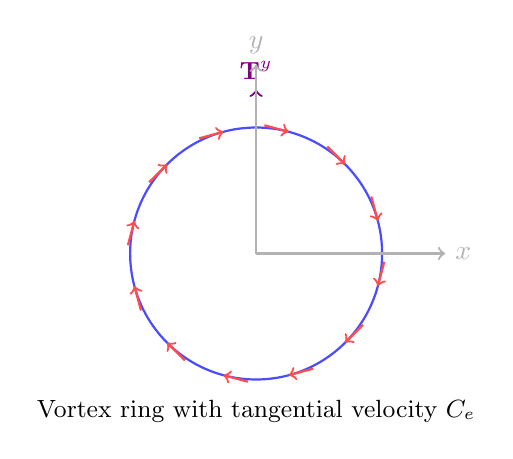
\begin{tikzpicture}[scale=0.8]
        % Ring (vortex core)
        \draw[thick, blue!70] (0,0) circle (2);

        % Flow lines (tangential swirl)
        \foreach \a in {15,45,75,105,135,165,195,225,255,285,315,345} {
            \draw[->, red!70, thick]
            ({2*cos(\a)}, {2*sin(\a)})
            ++({-0.4*sin(\a)}, {0.4*cos(\a)})
            -- ++({0.4*sin(\a)}, {-0.4*cos(\a)});
        }

        % Central torsion arrow
        \draw[->, thick, violet] (0,0) -- (0,2.6) node[above] {\small $\mathbf{T}^y$};

        % Axis labels
        \draw[->, thick, gray!60] (0,0) -- (3,0) node[right] {$x$};
        \draw[->, thick, gray!60] (0,0) -- (0,3) node[above] {$y$};

        % Label
        \node at (0,-2.5) {\small Vortex ring with tangential velocity $C_e$};
    \end{tikzpicture}
\end{center}


\noindent
This diagram shows a vortex ring in the $x$-$y$ plane with tangential swirl velocity (red arrows) and central torsion aligned along the $y$-axis,
representing $\mathbf{T}^y$ from Cartan's torsion 2-form.

\section{Physical Interpretation of the Æther}\label{sec:aether-interpretation}

In the Vortex \ae ther Model (VAM), the \ae ther is a physically real, incompressible, inviscid superfluid that fills all space and serves as the medium in which vortex structures propagate. Unlike the luminiferous æther of pre-relativistic physics, the VAM æther is not a rigid or preferred frame in the classical sense, but a \emph{relational fluid substrate} whose dynamics obey local conservation laws and whose properties are encoded in geometric field variables such as vorticity $\vec{\omega}$, swirl potential $\chi$, and pressure gradients $\nabla P$.

\subsection{Æther and Relativity}

Contrary to historical objections (e.g., Michelson--Morley), the VAM æther is consistent with observed relativistic invariance. In VAM:

\begin{itemize}
    \item The speed of light $c$ emerges as the limiting swirl propagation velocity in the æther.
    \item Time dilation and length contraction are derived from local swirl energy density~\cite{iskandarani2025b}, not from coordinate transformations.
    \item There is no global rest frame detectable through mechanical means, since only \emph{local} vorticity gradients affect physical observables.
\end{itemize}

This formulation parallels “emergent spacetime” scenarios in analogue gravity~\cite{barcelo2011}, where effective relativistic metrics arise from fluid microdynamics.

\subsection{Æther as a Relational Fluid}

The VAM æther is defined by its core properties:
\begin{itemize}
    \item \textbf{Incompressibility:} $\nabla \cdot \vec{v} = 0$
    \item \textbf{Inviscid Dynamics:} No intrinsic dissipation; supports persistent circulation.
    \item \textbf{Vortex-Centric Ontology:} All matter, radiation, and fields emerge as stable or propagating vortex excitations.
\end{itemize}

There is no absolute “grid” of space; instead, all physical quantities are encoded in the swirl structure of this medium. Thus, the æther is more akin to a quantum condensate than to a static frame, resembling ideas in superfluid vacuum theories~\cite{volovik2003}.

\subsection{Consistency with Experiments}

Although VAM includes a real æther, it remains consistent with all null results from first-order ether-drift experiments:

\begin{itemize}
    \item Light’s propagation is governed by local swirl—not frame-relative motion.
    \item The model predicts no Doppler shift or anisotropy in $c$ detectable in co-moving swirl regions.
    \item Apparent Lorentz invariance emerges as a \emph{symmetry of the equations} describing low-energy swirl excitations (e.g., vortex rings).
\end{itemize}

Thus, the æther in VAM functions as a hidden substrate—locally observable only through second-order effects like swirl-induced time dilation, vortex pressure gradients, or geometric birefringence in extreme fields.

\begin{quote}
        \emph{The VAM æther is a dynamic, relativistically compatible, vorticity-supporting fluid---not a classical rest frame.}
\end{quote}